\documentclass[border=10pt]{standalone}

\usepackage{tikz}
\usepackage{tikzsymbols}
\usetikzlibrary{calc,patterns,shapes.geometric}

\def\centerarc[#1](#2)(#3:#4:#5){\draw[#1] ($(#2)+({#5*cos(#3)},{#5*sin(#3)})$) arc (#3:#4:#5);}

\begin{document}
	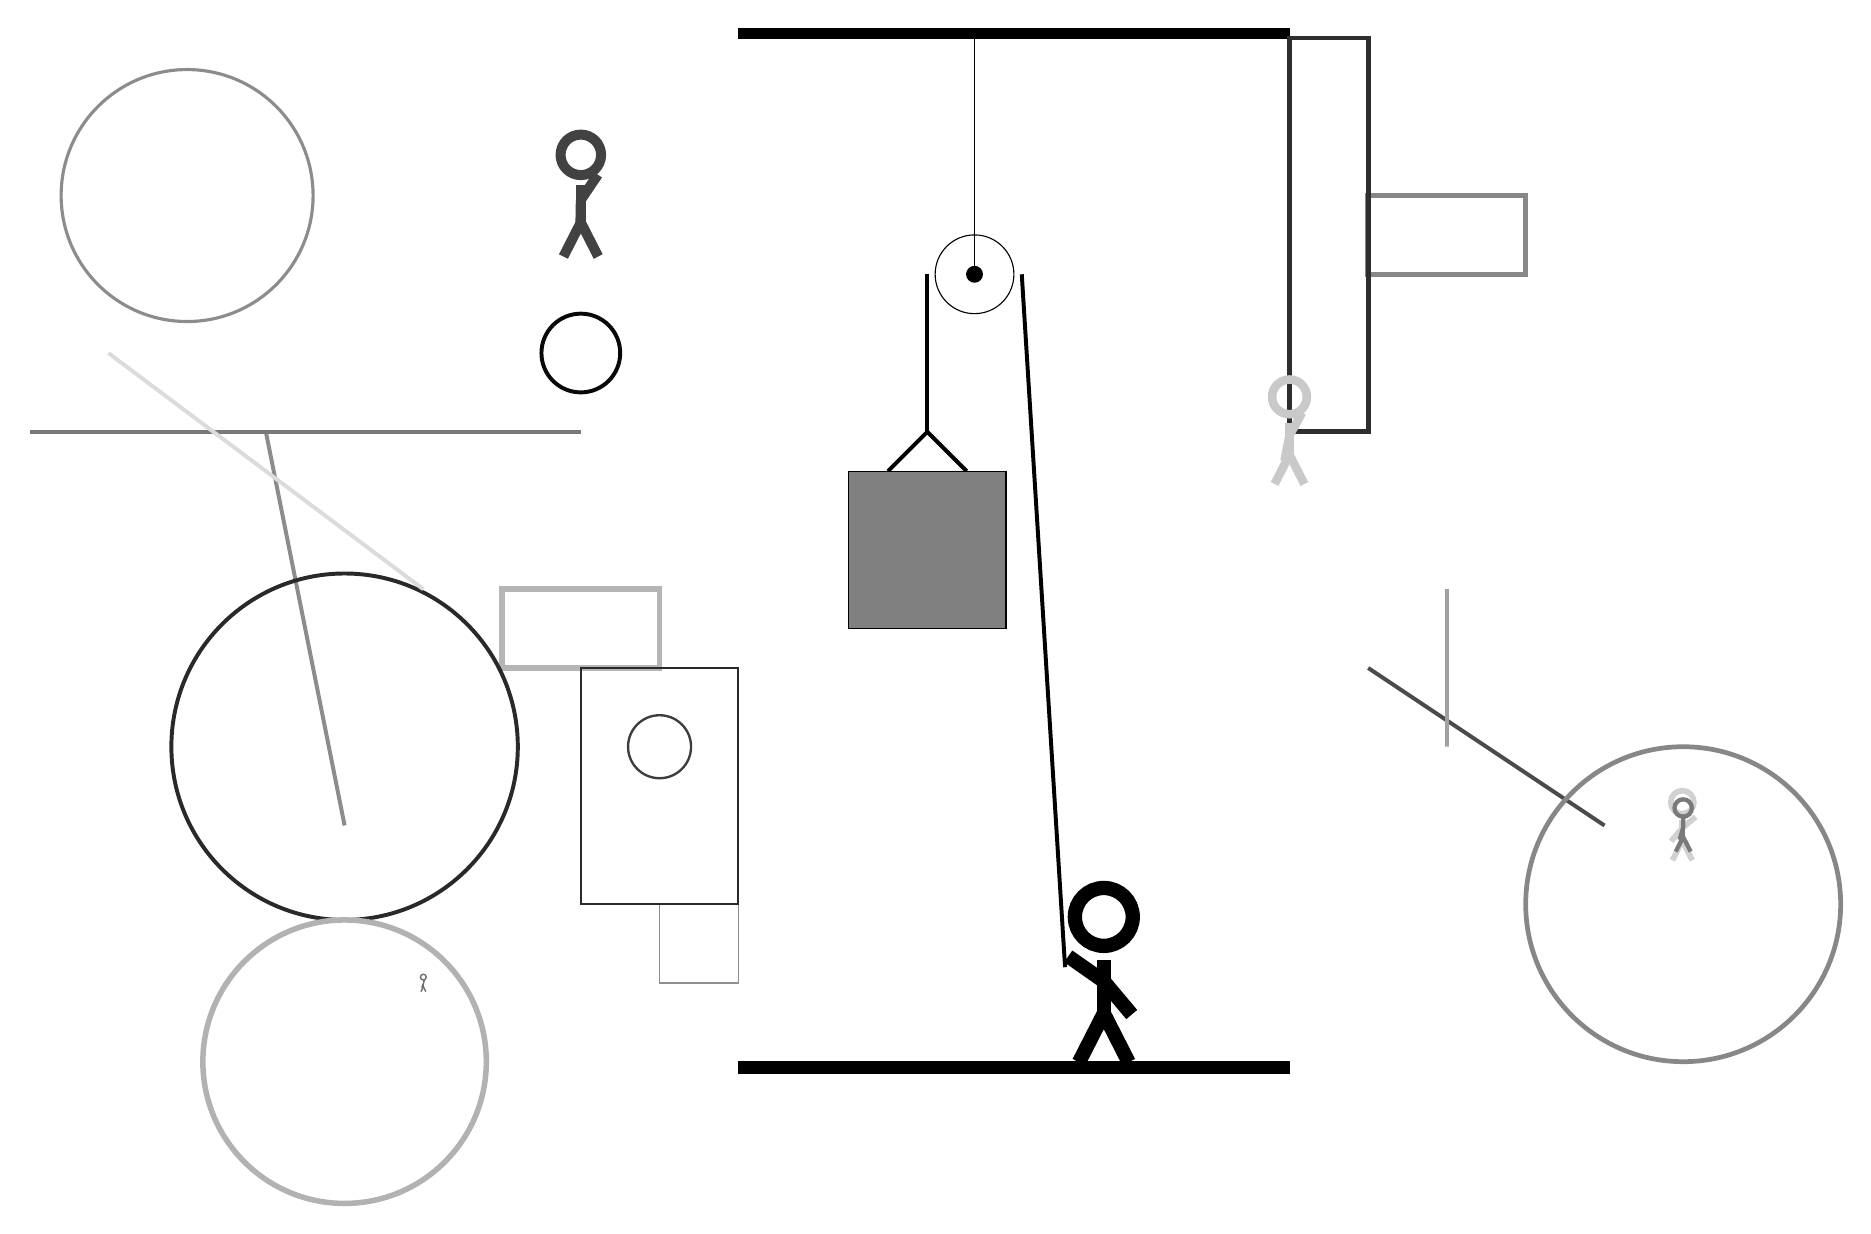
\begin{tikzpicture}
		%%%%% START %%%%%
		
		\draw[fill=black] (-2, 10) rectangle (5, 10.125);
		
		\draw (1, 7) circle (0.5);
		\draw[fill=black] (1, 7) circle (0.1);
		\draw (1, 10) -- (1, 7);
		
		\draw[line width=0.5mm] (-0.1, 4.5) -- (0.4, 5.0) -- (0.9, 4.5);
		\draw[fill=black!50] (-0.6, 4.5) rectangle (1.4, 2.5);
		
		\draw[line width=0.7mm, color=black!29] (-3, 2) rectangle (-5, 3);
		
		\draw[line width=0.2mm, color=black!44] (-3, -2) rectangle (-2, -1);
		\draw [line width=0.4mm, color=black!45](-9, 8) circle (1.6);
		\draw[line width=0.3mm, color=black!84] (-2, -1) rectangle (-4, 2);
		
		\draw[line width=0.5mm, color=black!45](-7, 0) -- (-8, 5);
		\node[line width=0.6mm, color=black!74] at (-4, 8) {\Strichmaxerl[7][89][56]};
		\draw [line width=0.5mm, color=black!97](-4, 6) circle (0.5);
		\draw [line width=0.3mm, color=black!76](-3, 1) circle (0.4);
		\draw [line width=0.5mm, color=black!84](-7, 1) circle (2.2);
		\node[line width=0.7mm, color=black!57] at (-6, -2) {\Strichmaxerl[1][68][73]};
		
		\node[line width=0.7mm, color=black!18] at (10, 0) {\Strichmaxerl[4][50][40]};
		
		\draw[line width=0.5mm, color=black!71](6, 2) -- (9, 0);
		\draw[line width=0.7mm, color=black!47] (6, 7) rectangle (8, 8);
		\draw[line width=0.5mm, color=black!53](-4, 5) -- (-11, 5);
		\draw[line width=0.6mm, color=black!37] (7, 1) rectangle (7, 3);
		\draw[line width=0.6mm, color=black!82] (6, 5) rectangle (5, 10);
		
		\draw [line width=0.6mm, color=black!47](10, -1) circle (2.0);
		
		\node[line width=0.3mm, color=black!52] at (10, 0) {\Strichmaxerl[3][74][89]};
		\draw[line width=0.5mm, color=black!14](-6, 3) -- (-10, 6);
		\draw [line width=0.7mm, color=black!30](-7, -3) circle (1.8);
		\node[line width=0.5mm, color=black!21] at (5, 5) {\Strichmaxerl[6][79][61]};
		
		\draw[line width=0.5mm] (0.4, 7) -- (0.4, 5.0);
		\centerarc[line width=0.5mm](1, 7)(0:180:0.6);
		\draw[line width=0.5mm](1.6, 7) -- (2.15, -1.8);
		
		\node at (2.6, -1.9) {\Strichmaxerl[10][-35][-50]};
		
		\draw[fill=black] (-2, -3) rectangle (5, -3.15);
		
		%%%%% END %%%%%
	\end{tikzpicture}
\end{document}